\documentclass[11pt]{article}

\usepackage{amsmath,mathtools,siunitx}
\usepackage[a4paper,left=1.5cm,right=1.5cm,top=2cm,bottom=2cm]{geometry}
\usepackage{float,subcaption,graphicx}
\usepackage{enumitem,pifont}
\renewcommand{\labelitemi}{\ding{228}}
\renewcommand{\labelitemii}{\ding{229}}
\renewcommand{\labelitemiii}{\ding{225}}
\setlist[itemize]{noitemsep}
\usepackage[dvipsnames]{xcolor}
\usepackage{color,hyperref}
\hypersetup{colorlinks=true}

\newcommand{\tVVt}{\frac{|\tilde{V}_{ij}|^2}{|V_{ij}|^2}}
\newcommand{\tVV}{\frac{|\tilde{V}_{ij}|}{|V_{ij}|}}

\begin{document}
{\Large\bfseries Some notes on CKM element stuff}
\begin{itemize}
    \item So we have the usual BR description in 2HDM:
        \begin{equation*}
            \mathcal{B}r_{exp} = \mathcal{B}r_{SM}\times(1+r_H)^2
        \end{equation*}
    \item Here, $(1+r_H)^2$ describes the WC terms, and the CKM element is part of the SM equation, but if the 2HDM is correct, then what we get from experiment for the value of $|V_{ij}|^2$ is really $|V_{ij}|^2\times(1+r_H)^2$
        \begin{itemize}
            \item $r_H=0$ means that 2HDM is wrong, and we're back to the SM value being correct
            \item $r_H=-2$ means we're in the fine-tuned solution of the 2HDM and what we measure as the SM CKM element is the correct value, although the 2HDM is still correct
            \item $r_H\neq0,-2$ means that the real CKM element is different from the measured one and we can't use the given SM values
        \end{itemize}
    \item So if we assume 2HDM to be right, we're probably using the wrong CKM element
    \item Now consider having
        \begin{equation*}
            \mathcal{B}r_{exp} = \mathcal{B}r_{SM}\times\tVVt(1+r_H)^2
        \end{equation*}
        as our equation, with $\tilde{V}_{ij}$ being the `real' CKM element value and $V_{ij}$ being the measured one in the SM
    \item This lets us cancel the SM CKM value and input the `real' one, if there is a difference in their value
    \item For working in flavio, we need to write any modifications to SM formulae as NP WCs to be added to the SM WCs, so we need to rewrite this:
        \begin{align*}
            \tVVt(1+r_H)^2 &= \left\{\tVV+\tVV r_H\right\}^2 \\
                           &= \left\{1+\left(\tVV-1\right)+\tVV r_H\right\}^2
        \end{align*}
    \item Writing like this means we can just add on $\tVV-1$ to a WC (e.g. to \textbf{CVL\_bumunumu} in \href{https://wcxf.github.io/assets/pdf/WET.flavio.pdf}{flavio's WET basis} for $B^+\to\mu^+\nu_\mu$) and just multiply the WCs involved with $r_H$ by $\tVV$ 
    \item If the CKM element is not changed in the 2HDM, its contribution to the above will go away and we'll be back to our original consideration for the 2HDM; if it is changed, then we will be able to notice it
    \item This leaves us with 3 free parameters to fit, and I'm not sure if we can do that properly within flavio as it is, but it is simple enough to build up a picture of this modification's impact by doing a range of 2D contours as before for various values of $\tVV$
    \item The issue with this is that then you have to fit for each quark current so that you're only considering a single CKM element at once, and for some, i.e. kaons and pions, their errors in form factors are quite large so I'm not sure if we can really resolve much information from those fits
    \item I've done some quick contours for various values of $\tVV$ for the leptonic decays we've been using, which you can look through at \href{https://github.com/mbr-phys/higgs-proj/tree/master/ckm_tests}{github/mbr-phys/higgs-proj/tree/master/ckm\_tests} in individual folders for each CKM element consider
    \item It would probably be worthwhile adding more leptonic decays to these fits for better indication of our validity of choice in $\tVV$ but I haven't looked into any extras yet
    \item Using our leptonic decays so far, we can analyse how Vud, Vus, Vub, Vcd, and Vcs can be modified in the 2HDM, but for the other elements, we would have to extract from unitarity 
        \begin{itemize}
            \item We have all the first row elements here which means we could use unitarity as an extra constraint and test the elements together
            \item It might be possible to do similar to above for $\mathcal{R}(D^{(*)})$ and Vcb so we could then use unitarity constraints on the first two rows
        \end{itemize}
    \item Since $\gamma$ comes from the phase of the elements, it shouldn't be affected by the 2HDM, so while just considering 2HDM, we can use the usual method to construct the full matrix from knowing how to modify Vub, Vcb, Vus
    \item Here's how the leptonics change for Vub and Vus from some of the quick plots ($\tVV$ increasing as you go down the page):
\end{itemize}

\begin{figure}[H]
    \centering
    \begin{subfigure}[b]{0.45\textwidth}
        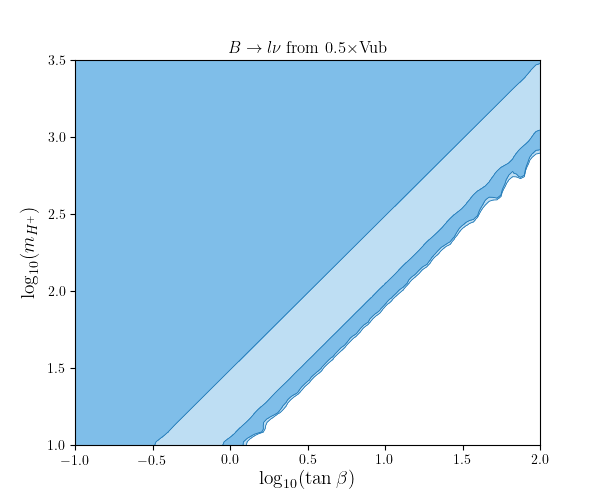
\includegraphics[width=\textwidth]{vub/Blnu0.5.png}
    \end{subfigure}
    \begin{subfigure}[b]{0.45\textwidth}
        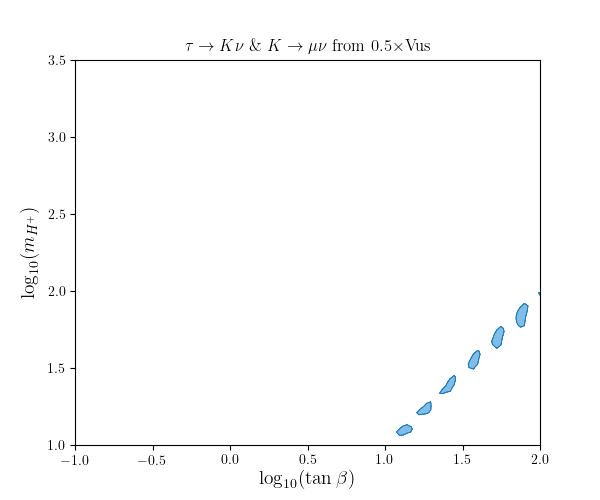
\includegraphics[width=\textwidth]{vus/Klnu0.5.png}
    \end{subfigure}
    \begin{subfigure}[b]{0.45\textwidth}
        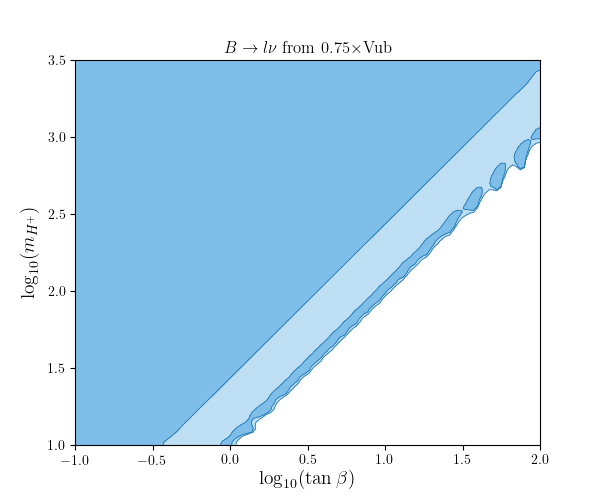
\includegraphics[width=\textwidth]{vub/Blnu0.75.png}
    \end{subfigure}
    \begin{subfigure}[b]{0.45\textwidth}
        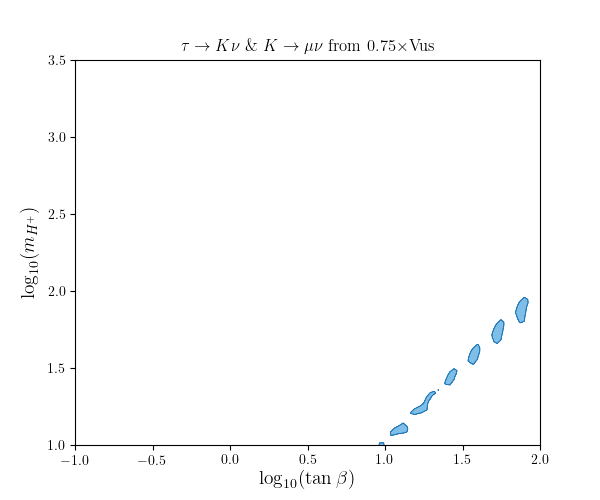
\includegraphics[width=\textwidth]{vus/Klnu0.75.png}
    \end{subfigure}
    \begin{subfigure}[b]{0.45\textwidth}
        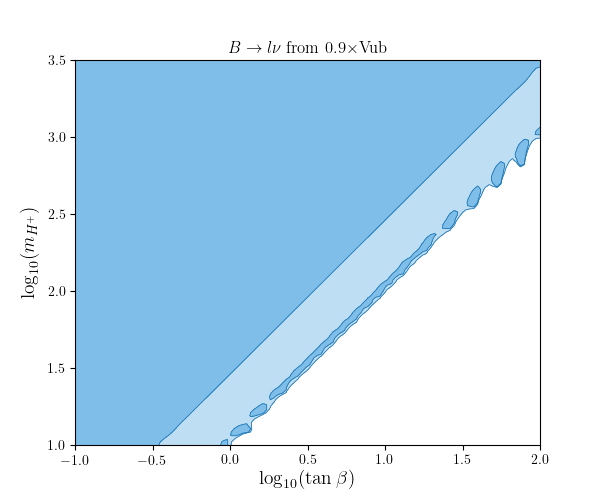
\includegraphics[width=\textwidth]{vub/Blnu0.9.png}
    \end{subfigure}
    \begin{subfigure}[b]{0.45\textwidth}
        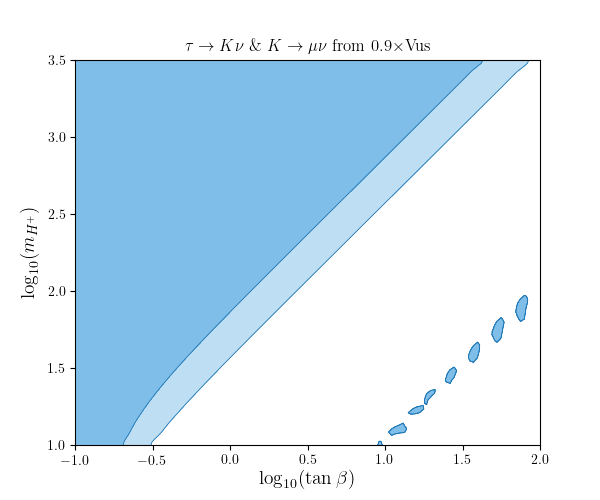
\includegraphics[width=\textwidth]{vus/Klnu0.9.png}
    \end{subfigure}
\end{figure}
\newpage
\begin{figure}[H]\ContinuedFloat
    \centering
    \begin{subfigure}[b]{0.45\textwidth}
        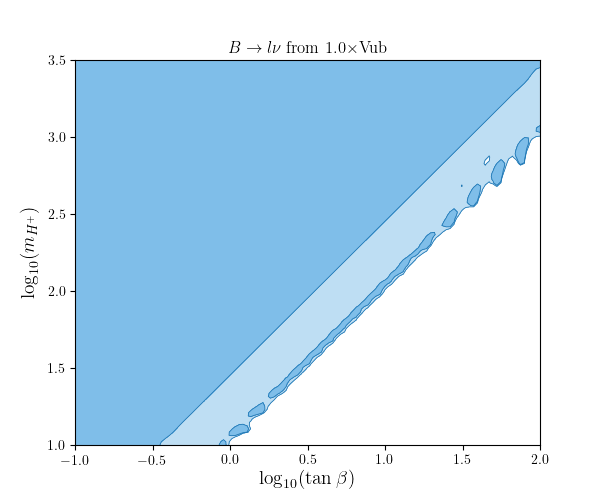
\includegraphics[width=\textwidth]{vub/Blnu1.0.png}
    \end{subfigure}
    \begin{subfigure}[b]{0.45\textwidth}
        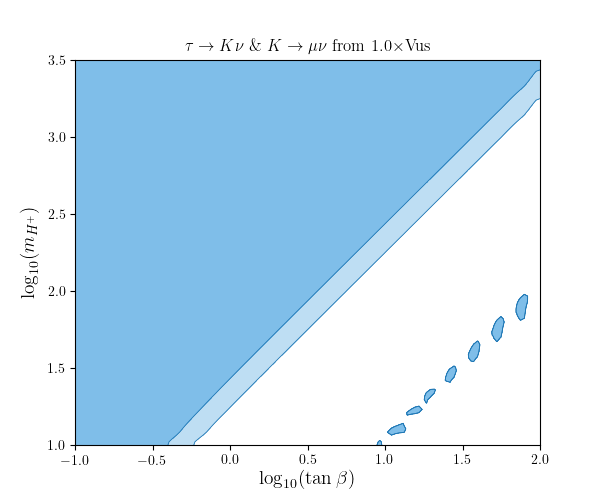
\includegraphics[width=\textwidth]{vus/Klnu1.0.png}
    \end{subfigure}
    \begin{subfigure}[b]{0.45\textwidth}
        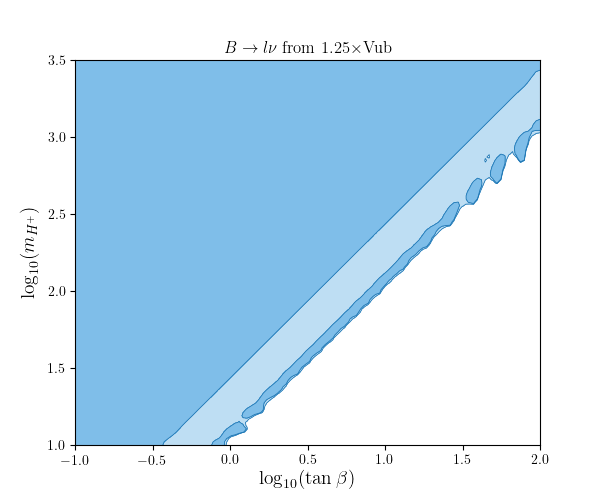
\includegraphics[width=\textwidth]{vub/Blnu1.25.png}
    \end{subfigure}
    \begin{subfigure}[b]{0.45\textwidth}
        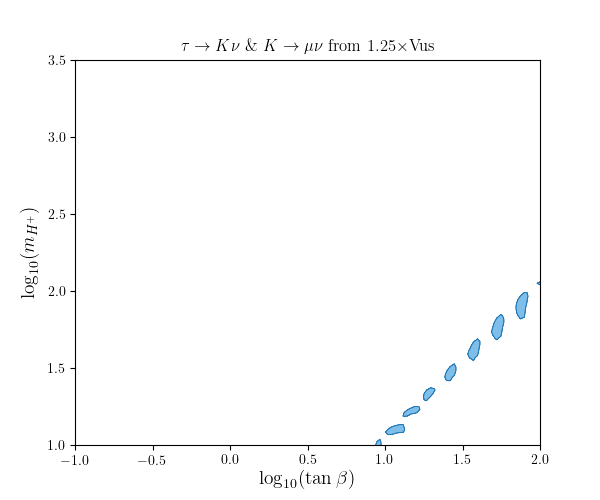
\includegraphics[width=\textwidth]{vus/Klnu1.25.png}
    \end{subfigure}
    \begin{subfigure}[b]{0.45\textwidth}
        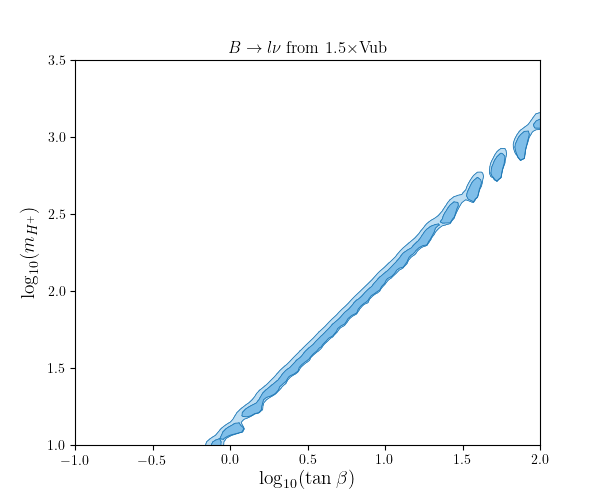
\includegraphics[width=\textwidth]{vub/Blnu1.5.png}
    \end{subfigure}
    \begin{subfigure}[b]{0.45\textwidth}
        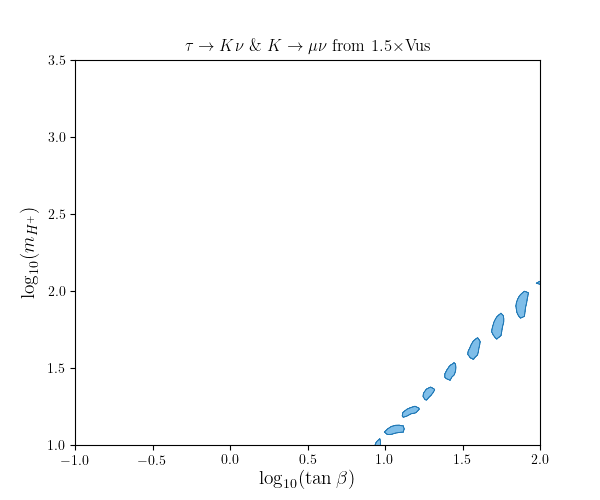
\includegraphics[width=\textwidth]{vus/Klnu1.5.png}
    \end{subfigure}
\end{figure}

\newpage
\begin{itemize}
    \item For leptonic decays, using $r_H$ as above, I've done some heatmaps showing values that $\tVV$ can take
    \item As James discussed in his notes, if the 2HDM is real then the value we measure and assume in the SM is
        \begin{align*}
            |V_{ij}|^2 = |\tilde{V}_{ij}|^2(1+r_H)^2 \implies \frac{1}{(1+r_H)} = \tVV
        \end{align*}
        So I have used this above for the following plots
    \item On the left are the plots across the full parameter space we've been using before; on the right are the plots in a reduced range for clarity - this region also corresponds to the approximate region seen in our usual plots for the leptonic decays
    \item Again, all plots and code are on the github link if you want to look closer
\end{itemize}

\begin{figure}[H]
    \centering
    \begin{subfigure}[b]{\textwidth}
        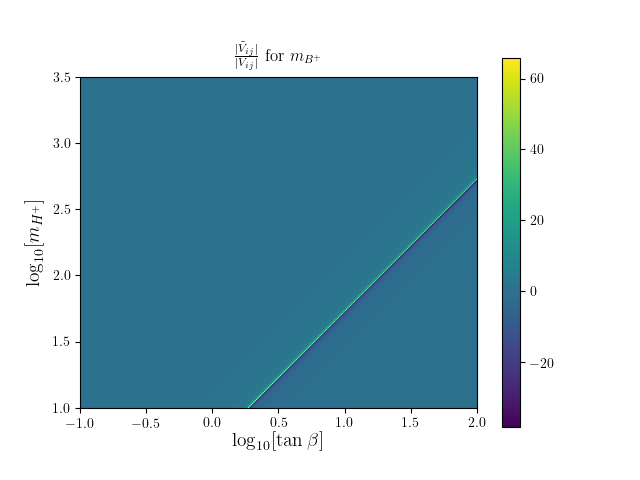
\includegraphics[width=0.49\textwidth]{heatmaps/mB-rH0.png}
        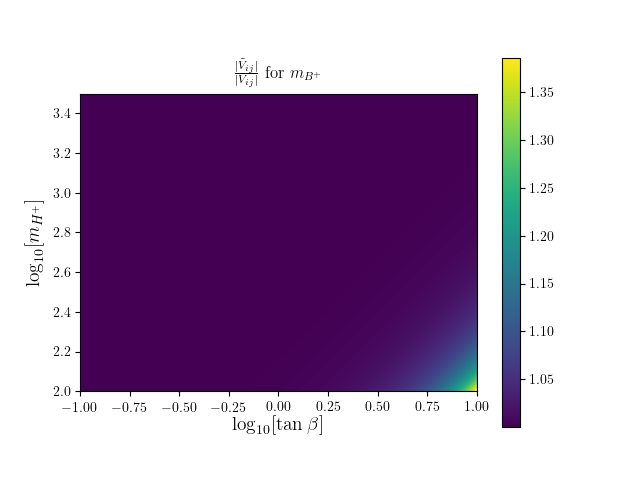
\includegraphics[width=0.5\textwidth]{heatmaps/mB-rH1.png}
        \caption{$m_{B^+} \implies V_{ub}$; on the right, the range is $\sim1\to1.4$}
    \end{subfigure}
    \begin{subfigure}[b]{\textwidth}
        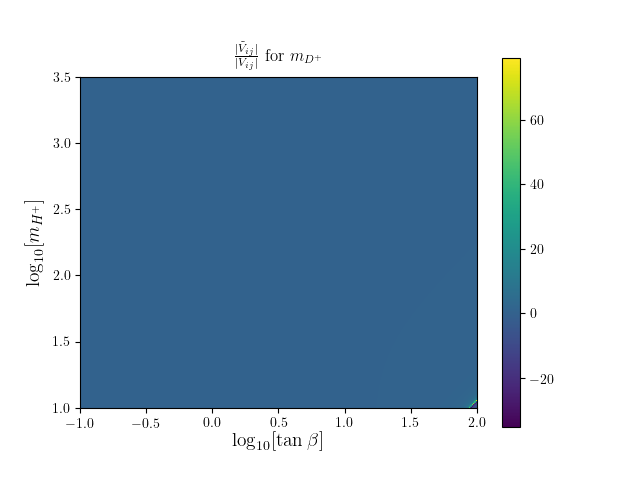
\includegraphics[width=0.49\textwidth]{heatmaps/mD-rH0.png}
        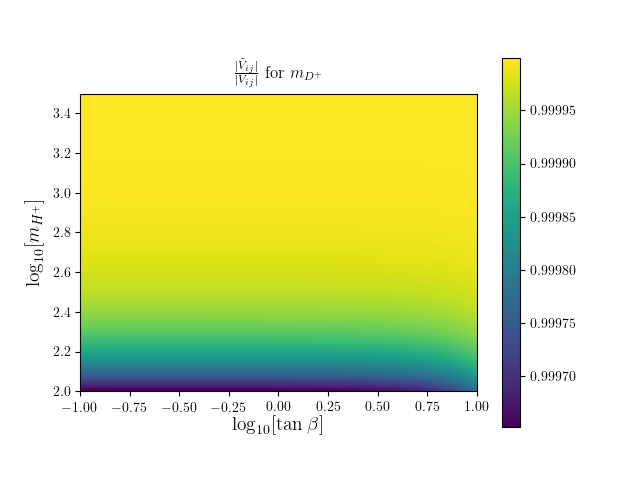
\includegraphics[width=0.5\textwidth]{heatmaps/mD-rH1.png}
        \caption{$m_{D^+} \implies V_{cd}$; on the right, the range is $\sim0.99965185\to0.99999978$}
    \end{subfigure}
\end{figure}
\newpage
\begin{figure}[H]\ContinuedFloat
    \centering
    \begin{subfigure}[b]{\textwidth}
        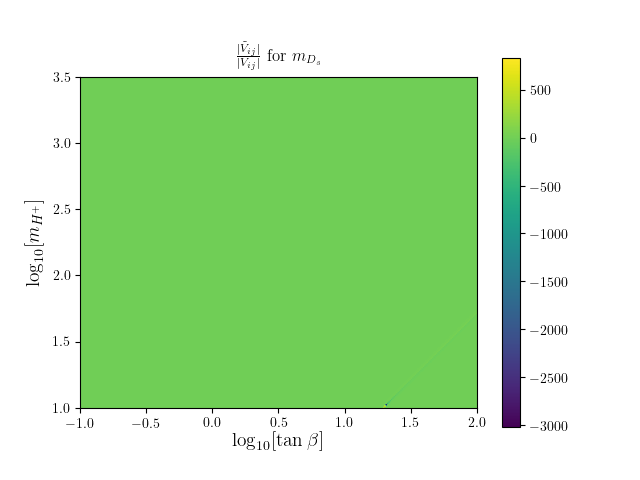
\includegraphics[width=0.49\textwidth]{heatmaps/mDs-rH0.png}
        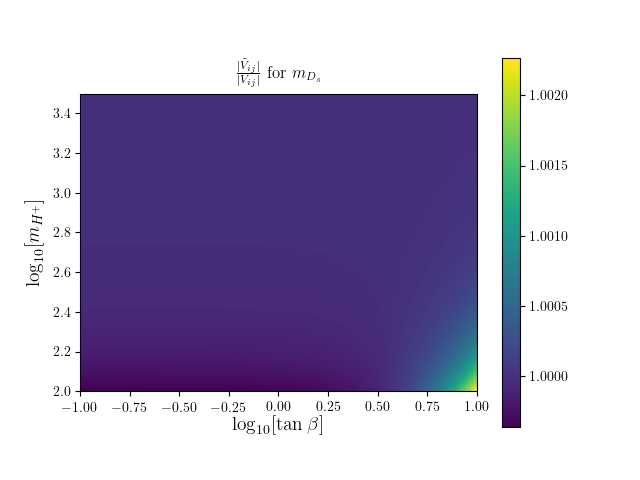
\includegraphics[width=0.5\textwidth]{heatmaps/mDs-rH1.png}
        \caption{$m_{D_s} \implies V_{cs}$; on the right, the range is $\sim0.99964\to1.00227$}
    \end{subfigure}
    \begin{subfigure}[b]{\textwidth}
        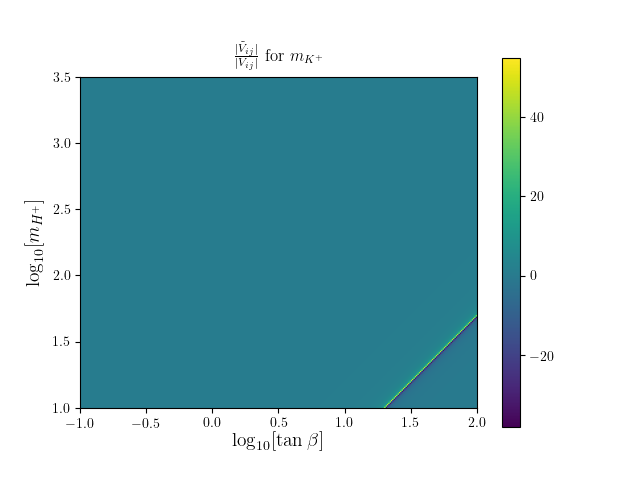
\includegraphics[width=0.49\textwidth]{heatmaps/mK-rH0.png}
        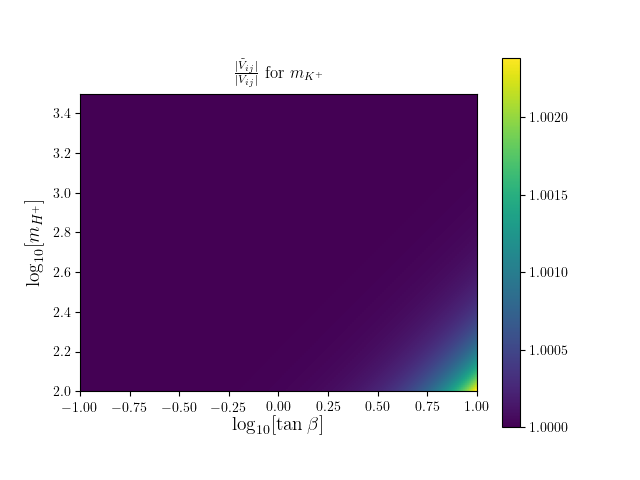
\includegraphics[width=0.5\textwidth]{heatmaps/mK-rH1.png}
        \caption{$m_{K^+} \implies V_{us}$; on the right, the range is $\sim0.9999997\to1.002386$}
    \end{subfigure}
    \begin{subfigure}[b]{\textwidth}
        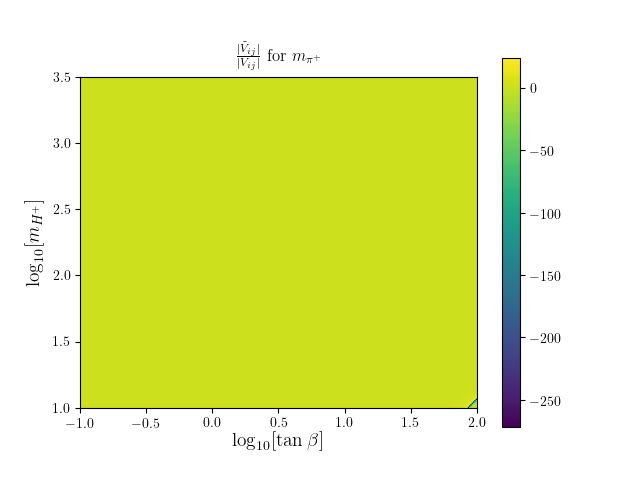
\includegraphics[width=0.49\textwidth]{heatmaps/mpi-rH0.png}
        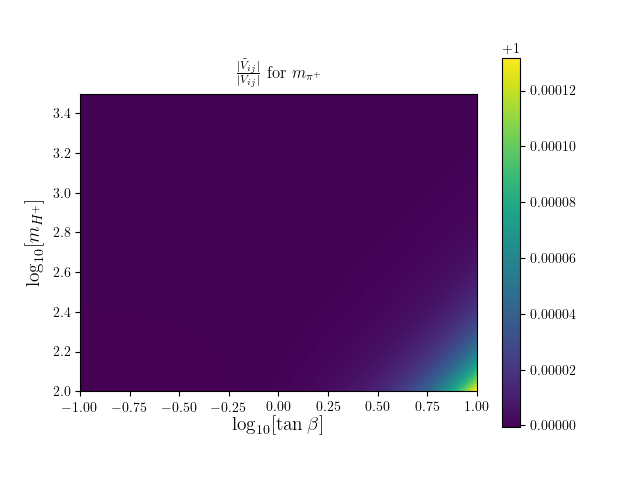
\includegraphics[width=0.5\textwidth]{heatmaps/mpi-rH1.png}
        \caption{$m_{\pi^+} \implies V_{ud}$; on the right, the range is $\sim0.9999994\to1.000132$}
    \end{subfigure}
\end{figure}
\textit{It's a bit unclear for the right hand diagram for $\pi^+$, but the values along the colourbar are all 1+ that value}

\newpage
\begin{itemize}
    \item For each point in parameter space, I have taken the modification factors for each CKM element from the heatmaps, modified the accepted CKM elements accordingly, and tested for unitarity in the first two rows
    \item I haven't looked at any modification of $V_{cb}$ yet either from building a similar sort of heatmap if possible from semileptonics, or using $B_c$ leptonic decays (though I don't know if there's enough data to use these)
\end{itemize}

\begin{figure}[H]
    \centering
    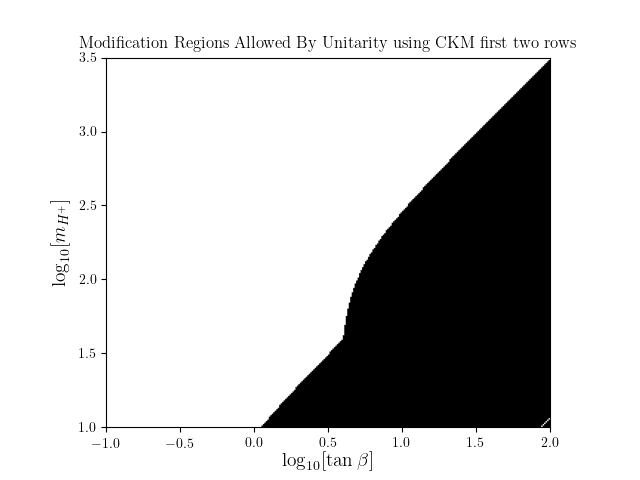
\includegraphics[width=0.49\textwidth]{heatmaps/ckm_mod_errs.png}
    \caption{The black region represents areas where the first two rows of the CKM matrix break unitarity from 2HDM modification as discussed above.}
\end{figure}

\end{document}












